\documentclass[14pt]{extarticle}
\oddsidemargin=0.0in
\evensidemargin=0.0in
\textwidth=6.5in
\topmargin=-0.75in
\textheight=9.5in
%\usepackage{hyperref}
\usepackage{url}
\usepackage{graphicx}
\usepackage{amsmath}

\begin{document}
\pagestyle{empty}
 
\begin{center}
{\LARGE {\bf Homework Nine}}\\
\bigskip
{\Large {\bf Calculus I}}\\
\bigskip
{\Large {\bf College of the Atlantic}}\\
\bigskip
{ {\bf Due Friday, November 11, 2022}}\\ 
\end{center}
\medskip

%\noindent There are two parts to this assignment.\\

\noindent {\bf Part 1: WeBWorK}.  Do Homework 08 on
WeBWorK.  The WeBWorK page is here: 
\url{https://webwork.runestone.academy/webwork2/coa-feldman-es1024i-fall-2022/}.
I recommend doing the WeBWorK part of the homework first.  This will
enable you to benefit WeBWorK's instant feedback before you do part
two.\\ 


\noindent {\bf Part 2: Non-WeBWorK problems}.  Here are some
instructions for how to submit this part of the assignment.
\begin{itemize}
  \setlength{\itemsep}{0mm}
\item Do the problems by hand using pencil (or pen) and paper.
  There is no need to type this assignment.
%\item If you like working on a tablet, go for it. 
\item Make a pdf scan of your work using genius scan or some
  similar scanning app.  Please make the homework into a single
  pdf, not multiple pdfs.
\item Submit the assignment on google classroom.  Please don't
  email it to me.
  %(Between my two classes I will be receiving
  %around 60 assignments a week.  Keeping track of them all in email 
  %is challenging.)
%\item If you want, you can do the non-WeBWorK problems in pairs and
%  submit only one assignment for the two of you. 
\end{itemize}

\noindent Here are some non-WeBWorK problems.


\begin{enumerate}
\setlength{\itemsep}{3mm}

\item You and your friend both traveled to Des Moines, Iowa, for a
fun-filled weekend get together. Monday morning comes and you head your
separate ways. You drive due north toward Minneapolis at 100 km/hr,
and your friend drives due west toward Omaha at 50 km/hr. As you head
northward, you think about how much you miss your friend, and you
picture them heading west, getting ever farther away from you. You
begin to wonder: how fast is the distance between me and my friend
growing?

\begin{enumerate}

  \item How fast is the distance between you and your friend growing
    after you have each been driving for one hour?
    
  \item How fast is the distance between you and your friend growing
    after you have each been driving for two hours? \\

\end{enumerate}




\item It is winter break and you are bored. You decide to pass the time by 
watching cars drive by on a lonely road near your home.  The road
happens to run directly east-west. You position yourself 5 meters
south of the road.

A car appears in the distance to your right. You watch it as it gets
closer and closer to you.  It passes directly in front of you and then
recedes to the left. Eventually it is so far away that you can no
longer see it.
This scene repeats itself several times over the next hour.  You begin
to wonder, how is the speed at which I have to move my head related to
how fast the car is going and the position of the car?

Let $\theta$ refer to the angle between your line of sight and due
east. So if you are looking due east, $\theta=0$, and if you are
looking due north, $\theta = \pi/2$.  On this road cars always travel
at a constant speed of 60 km/hr. 


\begin{enumerate}

\item You are watching a car.  At the moment in time at which
  $\theta=\pi/3$, at what rate (in radians/sec) must you turn your
  head so that the car remains in the center of your line of sight?

\end{enumerate}


\begin{figure}[h!]
\begin{center}
\vspace{-1mm}
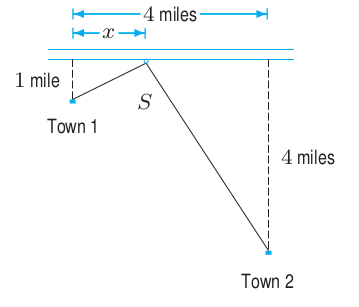
\includegraphics[width=3.7in]{towns.png}
\vspace{-2mm}
%\caption{The amount of energy used by a flying bird.}
\label{fig:towns}
\vspace{-15mm}
\end{center}
\end{figure}

\item Two towns are located near a straight river, as shown in the
  figure above. Town 1 is one mile from the river and town 2 is four
  miles from the river. The two towns both will get drinking water
  from a single pumping station, whose location is indicated by S on
  the figure. There will need to be a pipeline from the pumping
  station to each of the towns. Where should the pumping station be
  located so the length of the pipeline is minimized? 

\end{enumerate}

\end{document}




  \item Determine an equation for the linear function that generates
    the values in the table below.  

\begin{center}
\begin{tabular}{|| l | l ||}
\hline $x$ & $f(x)$ \\
\hline
5.2 & 27.8 \\
5.3 & 29.2 \\
5.4 & 30.6 \\
5.5 & 32.0 \\
5.6 & 33.4 \\
\hline
\end{tabular}
\end{center}





\end{document}
